% 第 15 章：格点理论中的相变
% 译自：extract/sec15.txt（PDF 第 93-97 页）+ 位于 extract/sec16.txt 开头的内容
% （PDF 第 98 页，在 "16. Errors in Lattice Results" 标题之前）。

\chapter{格点理论中的相变}

具有有限截断 $\mu = \pi/a$ 的格点理论可以视为一种有效理论。对动量区间 $\{\pi/a, \infty\}$ 内的积分使耦合常数重整化，并产生附加的有效相互作用（详见第 8 节以及 M.~L\"uscher 的讲义对这一方法的详细讨论）。因此，可以把格点理论看作无穷维耦合常数空间中的一个点，而取连续极限则是在这个空间中流向定义物理理论的 $a = 0$ 处临界点的流动。当人们以这种方式把格点QCD（LQCD）看作一个统计力学系统时，自然会引出以下问题
\begin{itemize}
\item 在这个扩展的耦合常数空间中，相图是什么样的？
\item 是否存在其他不动点？如果存在，这些点处理论的性质是什么？
\item 表征不同相的序参量是什么？
\end{itemize}

我讨论这些问题的出发点是纯规范理论。与前面一样，规范作用量的推广形式为
\begin{equation}
S_g = \beta \sum_{i,j} \sum_{\mu,\nu} \sum_x c_{i,j}\, \mathrm{Re}\, \mathrm{Tr}\, W^{i,j}_{\mu\nu}
\end{equation}
其中 $W^{i,j}_{\mu\nu}$ 中对 $i$ 的求和遍及所有可能的威尔逊圈，对 $j$ 的求和遍及圈的所有表示。$\beta$ 是总体耦合常数，$c_{i,j}$ 给出不同圈的相对强度。

相图的三个最简单的规范不变探针是（正如 Elitzur 所证明的 [37]，规范非不变量的期望值为零）
\begin{itemize}
\item 威尔逊圈：如第 14.2.1 节所讨论的，它们包含关于静态夸克之间势能的信息。
\item 威尔逊线/波利亚科夫线。它们测量孤立夸克的自由能。
\item 手征凝聚 $\langle \bar{\psi}\psi\rangle$。它提供关于自发手征对称性破缺下真空取向的信息。
\end{itemize}

在 $g \to \infty$ 的极限下，格点QCD可以用强耦合展开来分析，如第 14.2.2 节所讨论的。利用这些方法可以证明，在 $g \to \infty$ 的极限下，对所有规范群（$U(1)$ 和 $SU(N)$），威尔逊圈的期望值都具有面积律。由于电动力学（$U(1)$）并不禁闭，这一耦合常数区域不可能对应物理理论。换言之，在类似 $U(1)$ 这样的非禁闭理论中，应当存在一个将强耦合相与弱耦合相分开的相变。这一点对于 $U(1)$ 已经得到证实，既通过解析方法 [130]，也通过蒙特卡洛模拟 [131]。对于像 QCD 这样既具有禁闭又具有渐近自由的理论，我们需要知道参数空间的这两个区域是否解析相连。只要展开的有效范围给出足够大的重叠，就可以使用强耦合展开和弱耦合展开等解析方法；否则就需要非微扰方法。

为了针对 $SU(3)$ 解决这些问题，我在图~\ref{fig:14} 中展示了对于最简单的作用量——威尔逊方格作用量——方形圈 $\{\mathrm{Re}\,\mathrm{Tr}\, W^{i \times i}\}$ 作为耦合常数 $\beta$ 的函数的行为。图中还给出了 $O(\beta^5)$ 阶强耦合展开 [133]、$O(g^4)$ 阶弱耦合展开 [134] 及其蝌蚪图改进（TIPT）版本以作比较。这些数值数据表明，在弱耦合相与强耦合相之间存在一个光滑但陡峭的转变，即没有相变。这一交叉发生在 $5 \lesssim \beta \sim 6$ 的窗口内，较大的圈在略高的 $\beta$ 处变为微扰的。强耦合展开和弱耦合展开在这一区域都失效（对 TIPT 而言，只有在大圈时这一点才明显），因此数值方法是必不可少的。这样的分析是 Creutz 以及 Creutz、Jacobs 和 Rebbi 开创性工作的基础 [132]，他们证明了弦张力从强耦合行为到弱耦合行为的转变不需要相变。他们的计算提供了第一个线索：从 $\beta \gtrsim 6.0$ 的模拟中或许有可能以 $O(20\%)$ 的误差获得连续物理。

\begin{figure}[htbp]
\centering
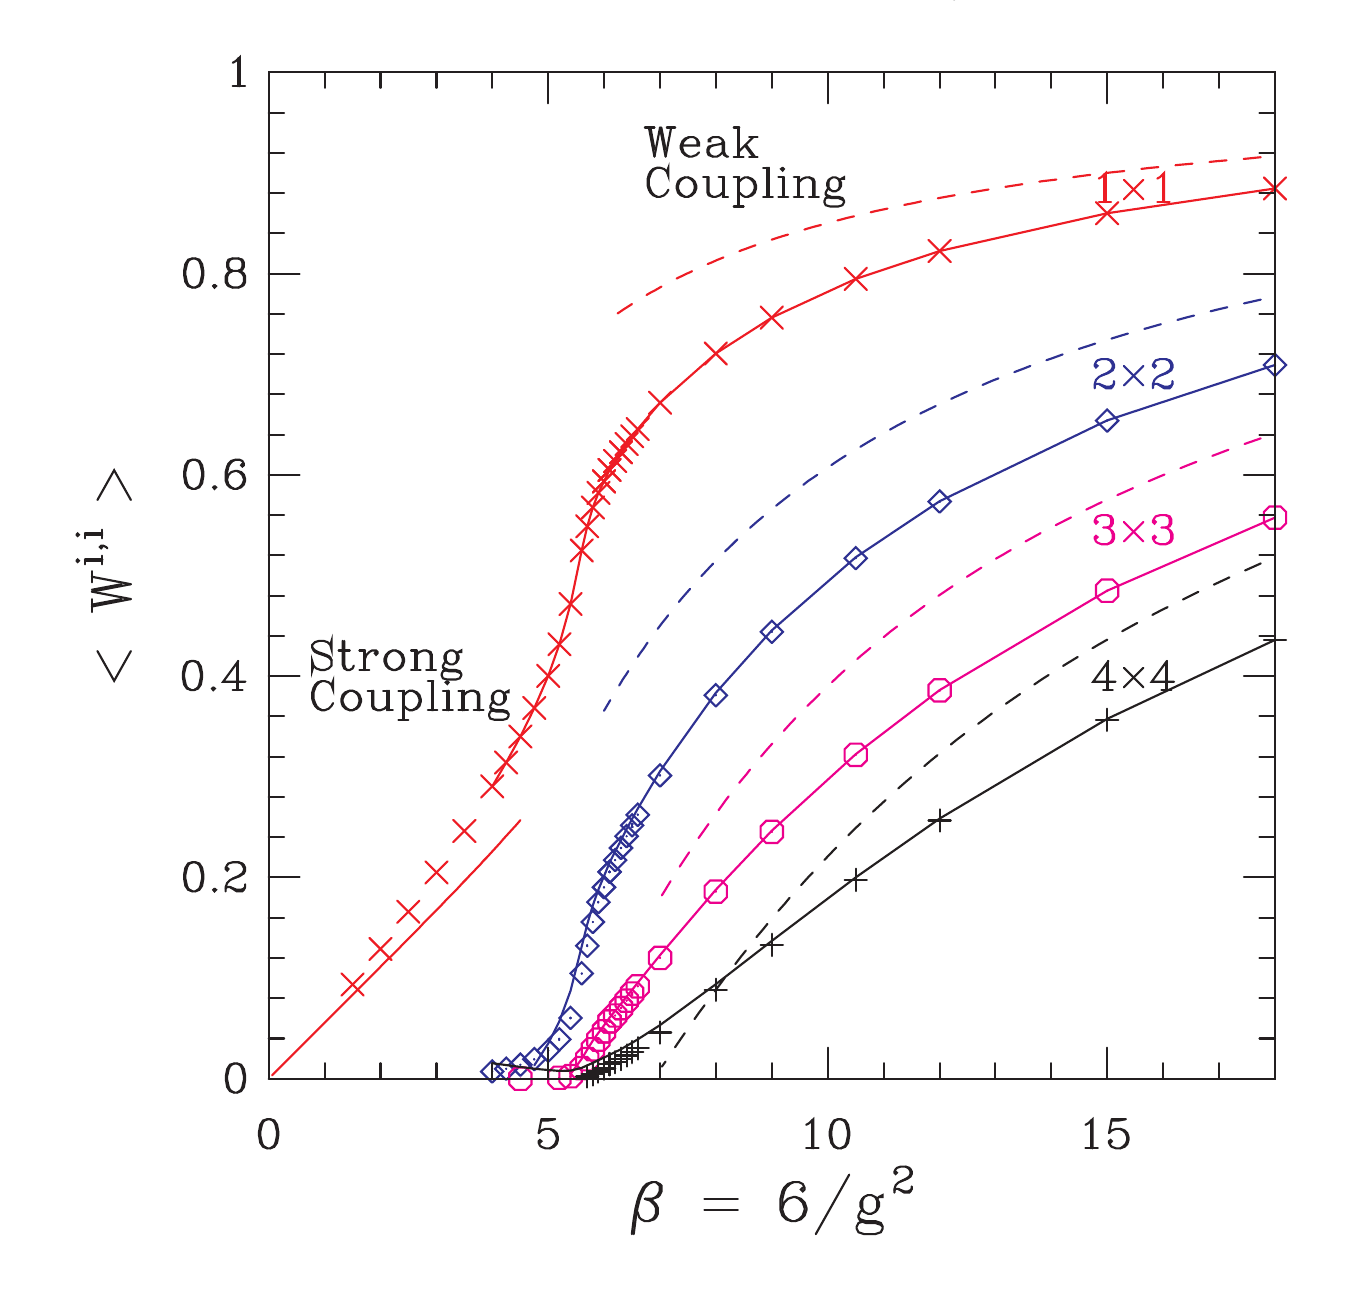
\includegraphics[width=0.8\textwidth]{images/fig14.png}
\caption{方形威尔逊圈期望值作为耦合常数 $\beta$ 的函数的行为。数据在 $5 \lesssim \beta \lesssim 6.0$ 之间显示出陡峭的交叉。虚线表示 $O(\beta^5)$ 阶强耦合展开和 $O(g^4)$ 阶弱耦合展开的结果。实线表示蝌蚪图改进的弱耦合展开（TIPT）的结果。由于改进的耦合常数是用 $1 \times 1$ 圈定义的，即 $g_I^2 = g^2/\langle W^{1 \times 1}\rangle$，数据与 TIPT 之间的一致性只是构造的平凡结果，如正文所述。然而，较大圈上的改进显示了 TIPT 的有效性。}
\label{fig:14}
\end{figure}

图~\ref{fig:14} 中显示的 TIPT 结果按如下方式获得。平均场改进的威尔逊圈期望值定义为
\begin{equation}
\langle W^{i \times i}\rangle = \langle \tilde{W}^{i \times i}\rangle\, u_0^{4i},
\end{equation}
其中 $u_0$ 我采用从方格获得的非微扰值，因为它更容易获得。在利用方格吸收蝌蚪图之后，$\langle \tilde{W}^{i \times i}\rangle$ 的改进展开由下式给出
\begin{equation}
\langle \tilde{W}^{i \times i}\rangle = \frac{\langle W^{i \times i}\rangle}{\langle W^{1 \times 1}\rangle^i},
\end{equation}
其中右边的两项首先按 $\tilde{g}^2 = g^2/u_0^4(\mathrm{pert}) = g^2/\langle W^{1 \times 1}\rangle_{\mathrm{pert}}$ 展开到 $\tilde{g}^4$ 阶，然后将比值截断在 $\tilde{g}^4$ 阶。显然，用来自方格的 $u_0$ 可以保证 $\langle W^{1 \times 1}\rangle$ 得到完美拟合，然而即使对 $\langle W^{4 \times 4}\rangle$ 的改进也是显著的。

对广义耦合常数空间中相图的首次研究，是使用由 $SU(N)$ 规范理论的基础表示和伴随表示中的方格构造的作用量进行的 [135]
\begin{equation}
S = \beta_F \sum_x \frac{1}{N} \mathrm{Re}\, \mathrm{Tr}\, W_{1 \times 1} + \beta_A \sum_x \frac{1}{N^2} |\mathrm{Tr}\, W_{1 \times 1}|^2 .
\end{equation}
对于这个作用量，用泰勒展开得到的有效裸耦合常数为
\begin{equation}
\beta_{\mathrm{eff}} \equiv \frac{2N}{g_{\mathrm{eff}}^2} = \beta_F + 2\beta_A .
\end{equation}
因此，只要 $\beta_F > 2|\beta_A|$，就可以在负 $\beta_A$ 区域进行模拟。这是一个避免弱耦合奇异性的经典条件。

所得的一级体相变线，连同三个规范群的端点位置，如图~\ref{fig:15} 所示。$\beta_A = \infty$ 处的点是 $Z(N)$ 规范理论中的一级相变，而 $\beta_F = 0$ 处的点对应 $SO(N)$ 理论中的一级相变。第三个端点相对于 $\beta_F$ 轴的位置取决于 $N$。目前对该位置的估计为 [136--138]
\begin{equation}
\begin{array}{lll}
\beta_F = 1.22 & \quad \beta_A = 1.25 & \quad \mathrm{SU}(2) \\
\beta_F = 4.00(7) & \quad \beta_A = 2.06(8) & \quad \mathrm{SU}(3) \\
\beta_F \sim 12{-}15 & \quad \beta_A = (-1) - (-5) & \quad \mathrm{SU}(4)
\end{array}
\end{equation}

对 $N \le 3$ 而言，该点位于 $\beta_F$ 轴上方，这一事实与图~\ref{fig:14} 所示威尔逊圈数据行为中没有间断的观测结果一致。如果沿一条在该点上方穿越转变线的路径取连续极限，例如沿图~\ref{fig:15} 中的虚线 $A$，那么在它与转变线的交点处，威尔逊圈（进而弦张力）、比热和胶球质量都会出现间断。在端点 $X$ 处比热发散，因此 $0^{++}$ 胶球质量趋于零。（注意，比热是以方格为插值算符的 $0^{++}$ 胶球关联函数的体积积分。因此比热的发散意味着 $0^{++}$ 胶球质量为零。）弦张力以及具有其他自旋-宇称量子数的胶球态的质量在该点处非零且连续。这类相变是格点人为效应。例如，在 $X$ 处取连续极限，即令 $a = 0$，将得到一个自由理论，因为除 $0^{++}$ 胶球外的所有态都变得无穷重。

\begin{figure}[htbp]
\centering
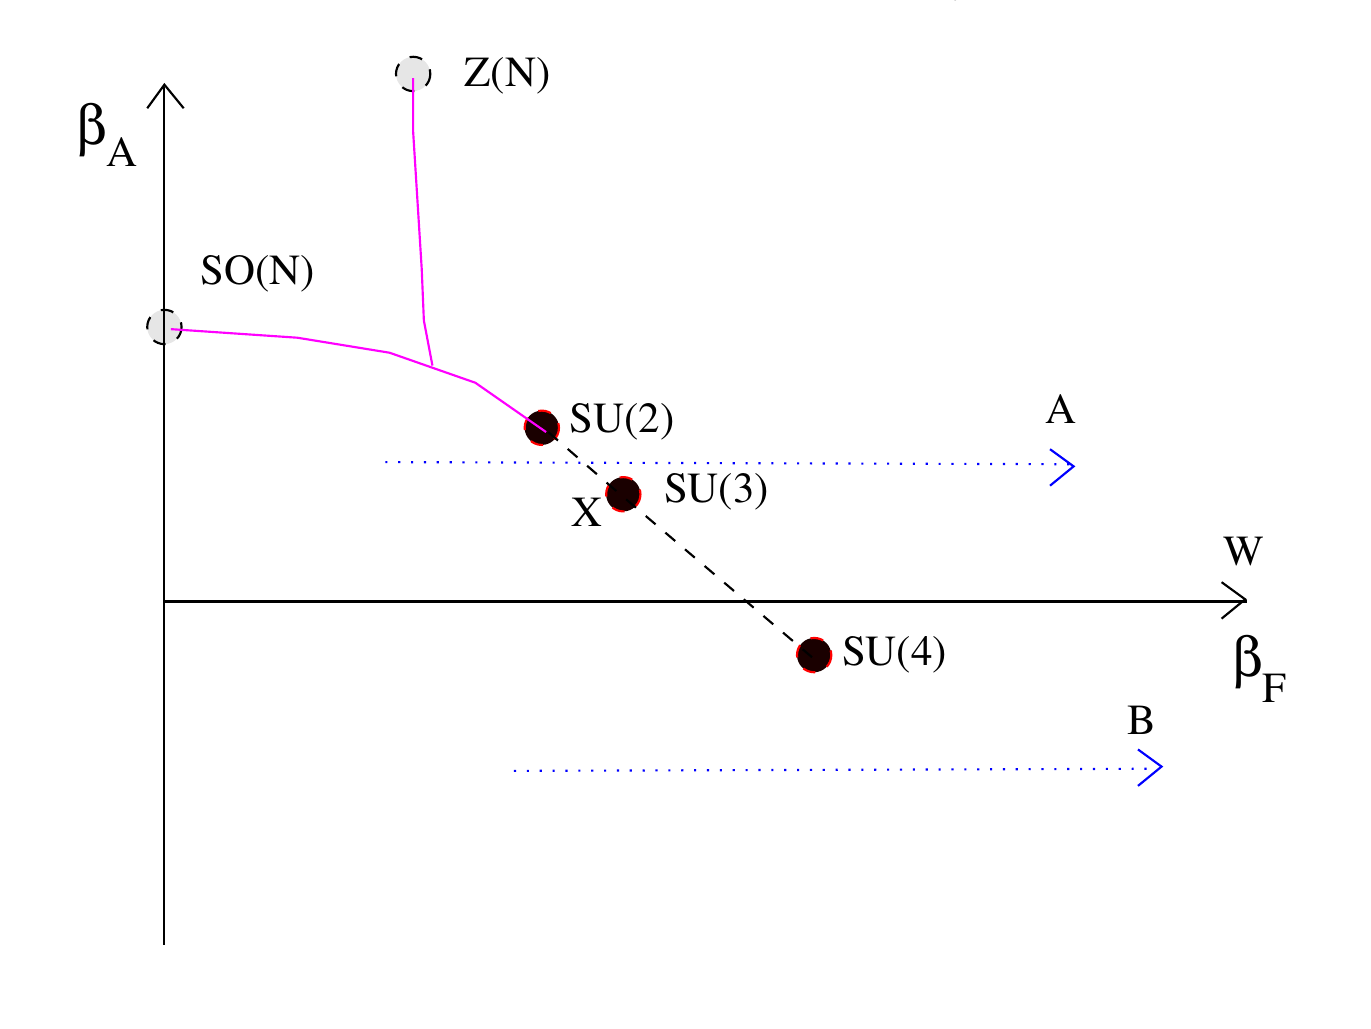
\includegraphics[width=0.8\textwidth]{images/fig15.png}
\caption{$SU(N)$ 规范理论在基础-伴随耦合常数空间中的相图。}
\label{fig:15}
\end{figure}

对于 $SU(3)$ 规范理论，可以沿诸如 $A$、$W$ 或 $B$ 这样的任何轨迹取连续极限。在情况 $A$ 中，必须保持 $\beta_F > \beta_F^*$ 以避免格点人为效应。沿 $W$，虽然没有奇异性，但人为效应 $X$ 在 $\beta_F = 5.7$ 附近可能引起对 $g = 0$ 处相关不动点物理的显著偏离。格点数据证实了这一情景——从 $M_{0^{++}}$ 以外的观测量测得的非微扰 $\beta$-函数在 $\beta_F = 5.7$ 附近显示出一个大的凹陷 [89]。因此，要避免这些人为效应需要 $\beta_F \gtrsim 6.0$ 的模拟。在像 $B$ 这样的轨迹上，预期 $X$ 的影响小于沿 $W$，并且在更粗的格点上就可能与连续物理建立联系。如果是这样，那么轨迹 $B$ 就对应一个符合第 8 节所列第三条判据的「改进作用量」。

这种沿像 $B$ 这样的轨迹取连续极限的定性论证，得到了对重整化轨迹的蒙特卡洛重整化群（MCRG）估计的支持 [87]。对重整化轨迹（RT）的这类计算给出 $\beta_A$ 为负值。如上所述，检验在作用量中加入 $\beta_A$ 项所预期改进的最敏感探针，是 $M_{0^{++}}$ 的行为。直到最近，对这一猜想的检验一直受限于统计精度 [166]。Morningstar 和 Peardon 最近在各向异性格点上对胶球谱的计算 [139] 证实了这一情景。我将在第 18.3 节讨论他们的结果。

显然，在广义格点理论中还存在其他相变。例如，如果作用量用基础表示和伴随表示中的 $1 \times 2$ 圈来定义，就会得到与图~\ref{fig:15} 类似的相图。因此，问题在于是否存在其他二阶相变点，在这些点上所有关联长度（以格点单位测量）都发散，即存在非平凡的连续极限。数值数据支持的一种普遍看法是，所有这些点都位于由 $g_{\mathrm{eff}} = 0$ 定义的超曲面上。这些理论的长距离行为由相对于合适的重整化群变换定义的不动点所控制。在这个超曲面上取格点理论的连续极限，提供了 QCD 的非微扰定义。这就是标准情景。

另一种情景是在 $g_{\mathrm{eff}} \neq 0$ 处存在非平凡不动点 [140]。如果这种可能性很小的情形被证明属实，那么基于渐近自由的 $g_{\mathrm{eff}}$ 与 $a$ 之间的微扰关系将会改变——随着动量标度 $Q \to \infty$，耦合常数将不再跑到零。这一点可以通过精确测量 $\alpha_s$ 作为 $Q^2$ 的函数来揭示，或者通过仔细搜寻格点理论中非平凡的二阶相变来揭示。

无论哪种情况，对诸如谱和弱矩阵元等量的非微扰格点分析都不会改变。为了达到连续极限，我们仍然要将格点数据在 $a$ 上外推到 $a = 0$。只有 $a$ 与 $g$ 之间的微扰QCD（PQCD）关系将失效，因此使用微扰标度关系的外推将不能再使用。

在提及了这种异端观点之后，我对此问题的结论是：继续假设标准情景是正确的来推进工作。
